\documentclass{beamer}
 
\usepackage[utf8]{inputenc}
\usepackage{amsmath}
\usepackage{amssymb}
 
 
%Information to be included in the title page:
\title{Ripple Tank}
\author{Ben Kettle}
\date{14 Jan 2020}
 
\begin{document}
 
\frame{\titlepage}

\begin{frame}{What is a Ripple Tank?}
    Today, we'll be using a ripple tank to demonstrate a few properties of waves. They're very simple, and consist of a few parts:
    
    \begin{itemize}
        \item Water Pool: A shallow pool of water with glass underneath.
        \item Lamp: A lamp from above allows us to see the wave shadows.
        \item Mirror $\&$ Projection Screen: for the light to hit.
        \item Wave Source: Either a point or linear source
        \item Power Source: Controls the way that the wave source moves
    \end{itemize}
    
    \vspace{5mm}
    
    Our ripple tank also has a \alert{strobe} that allows us to create a stationary image of the waves by matching the strobe frequency to the wave frequency. Thus, the waves are in the same position each time they are illuminated. 
\end{frame}

\begin{frame}{Linear Source: Basics}
    We can use a flat bar to form a linear wave. The ripple tank's power source pushes air through the hose periodically, moving the bar. 
    
    \begin{columns}[T]
         \begin{column}{.6\textwidth}
            Review: what should happen when we increase the frequency that the source moves? 
            \begin{itemize}
                \item Wave Frequency?
                \item Wavelength?
                \item Period?
            \end{itemize}
         \end{column}
         \begin{column}{.3\textwidth}
        \visible<2->{
           \begin{figure}
               \centering
               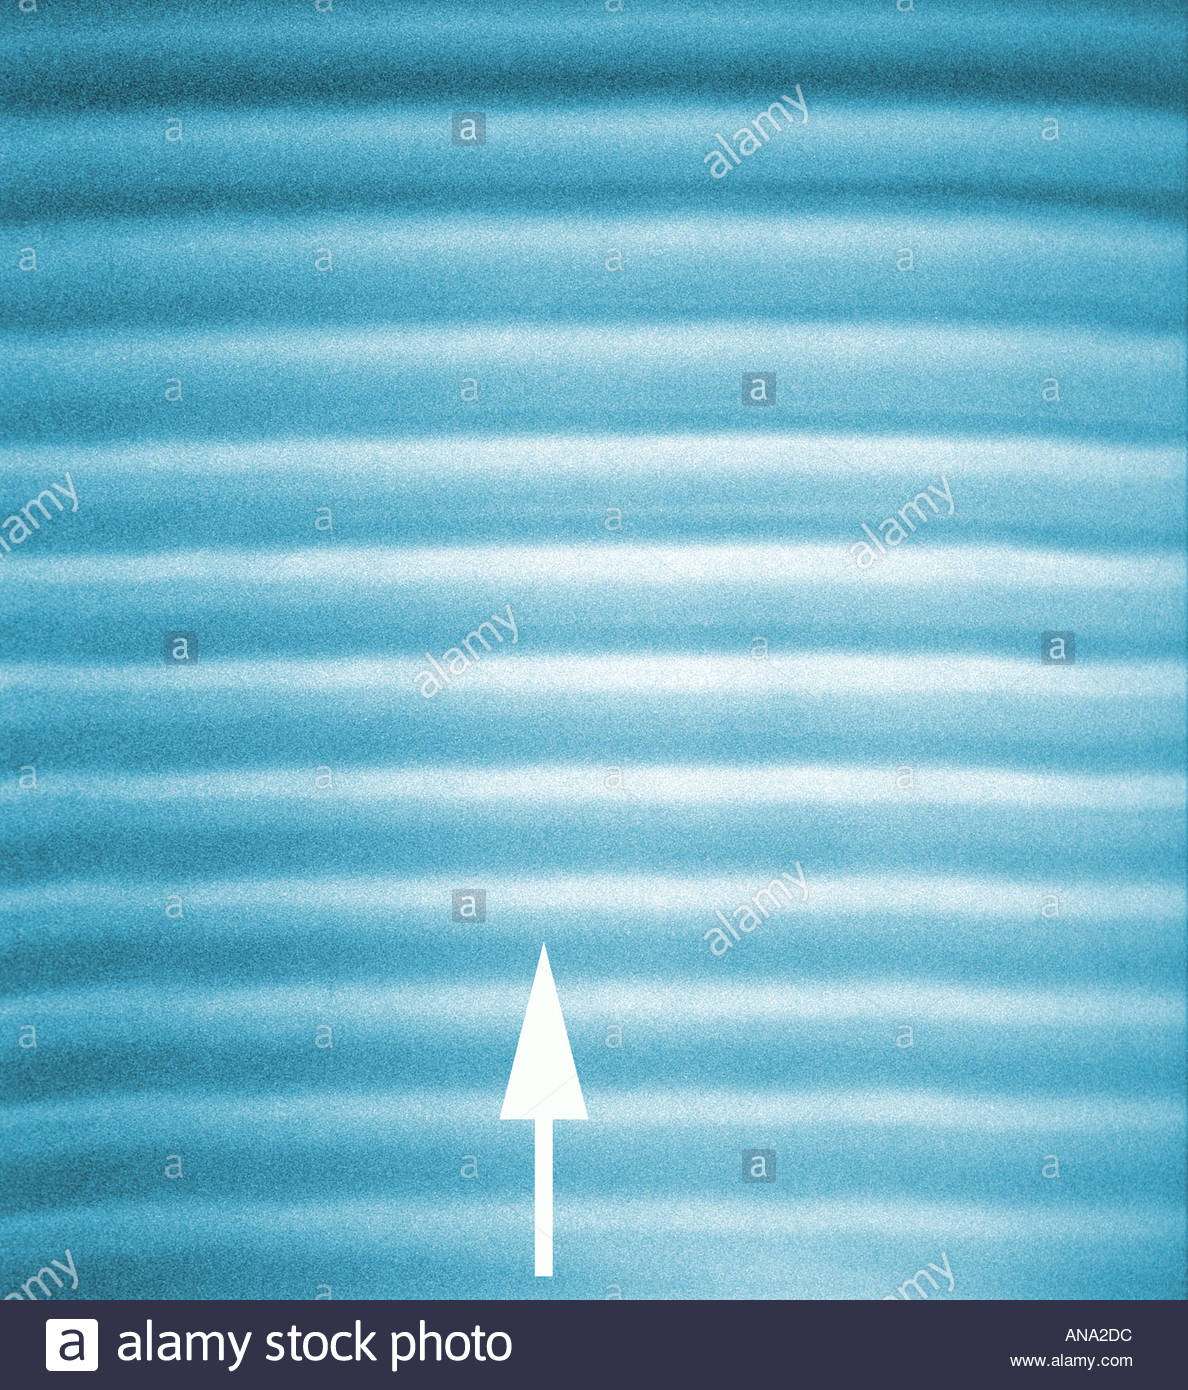
\includegraphics[scale=.07]{linearwaves.jpg}
               \caption{Linear waves in a ripple tank}
               \label{fig:linear}
           \end{figure}}
         \end{column}
    \end{columns}
\end{frame}

\begin{frame}{Linear Source: Reflection}
    If we add a flat object into the water, we can see waves reflect off of it. 
    \begin{itemize}
        \item What should the resulting pattern look like?
        \item Where will we see constructive interference?
        \item Where will there be destructive interference?
    \end{itemize} 
    \begin{columns}[T]
         \begin{column}{.45\textwidth}
            \visible<2->{
           \begin{figure}
               \centering
               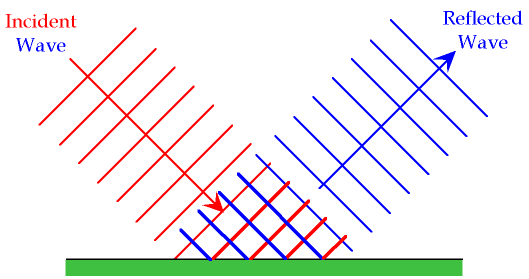
\includegraphics[scale=.26]{linreflect.png}
               \caption{Linear Wave Reflection}
               \label{fig:linref}
           \end{figure}}
         \end{column}
         \begin{column}{.45\textwidth}
            \visible<2->{\textbf{Let's try it!}}
            \visible<3->{
            \begin{figure}
               \centering
               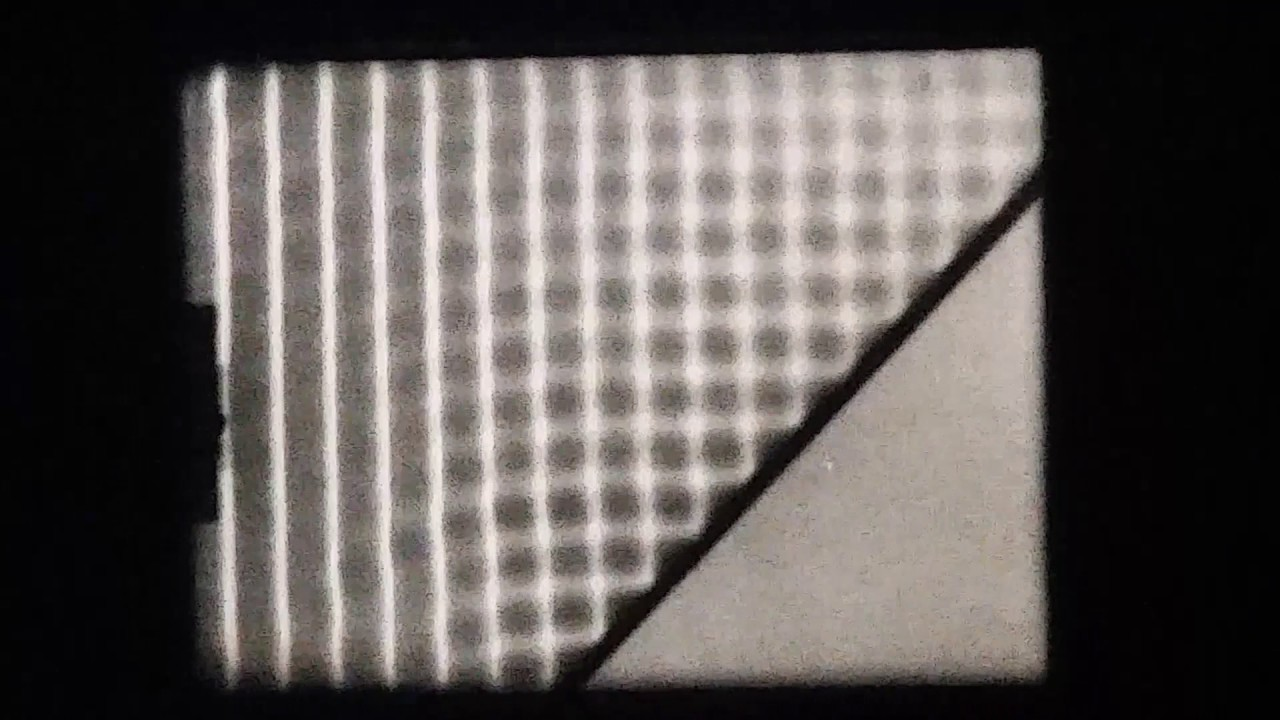
\includegraphics[scale=.1]{linrefripple.jpg}
               \caption{Linear Wave Reflection in a Ripple Tank}
               \label{fig:linrefripple}
           \end{figure}}
        \end{column}
    \end{columns}
\end{frame}

\begin{frame}{Linear Source: Reflection w/ Parabola}
    What if we use a parabolic reflector instead of a flat one? What effect will be created? Remember that waves will reflect \textit{across the normal}.
    \begin{columns}[T]
        \begin{column}{.45\textwidth}
            \begin{figure}
                \centering
                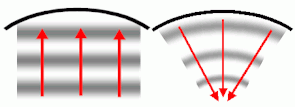
\includegraphics[scale=.45]{parabolaref.png}
                \caption{When waves reflect off of a parabola, they are focused into a single point.}
                \label{fig:parabolatheory}
            \end{figure}
        \end{column}
         \begin{column}{.45\textwidth}
           \begin{figure}
               \centering
               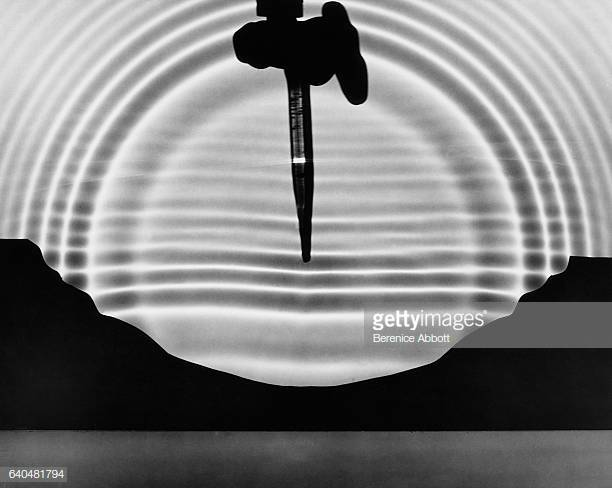
\includegraphics[scale=.7]{parabolaref2.jpg}
               \caption{Linear waves reflect off a parabola to form radial waves.}
               \label{fig:parabolatank}
           \end{figure}
         \end{column}
    \end{columns}
\end{frame}

\begin{frame}{Diffraction: Review}
    \alert{Diffraction} occurs when a wave encounters an object or a slit. 
    \begin{figure}
       \centering
       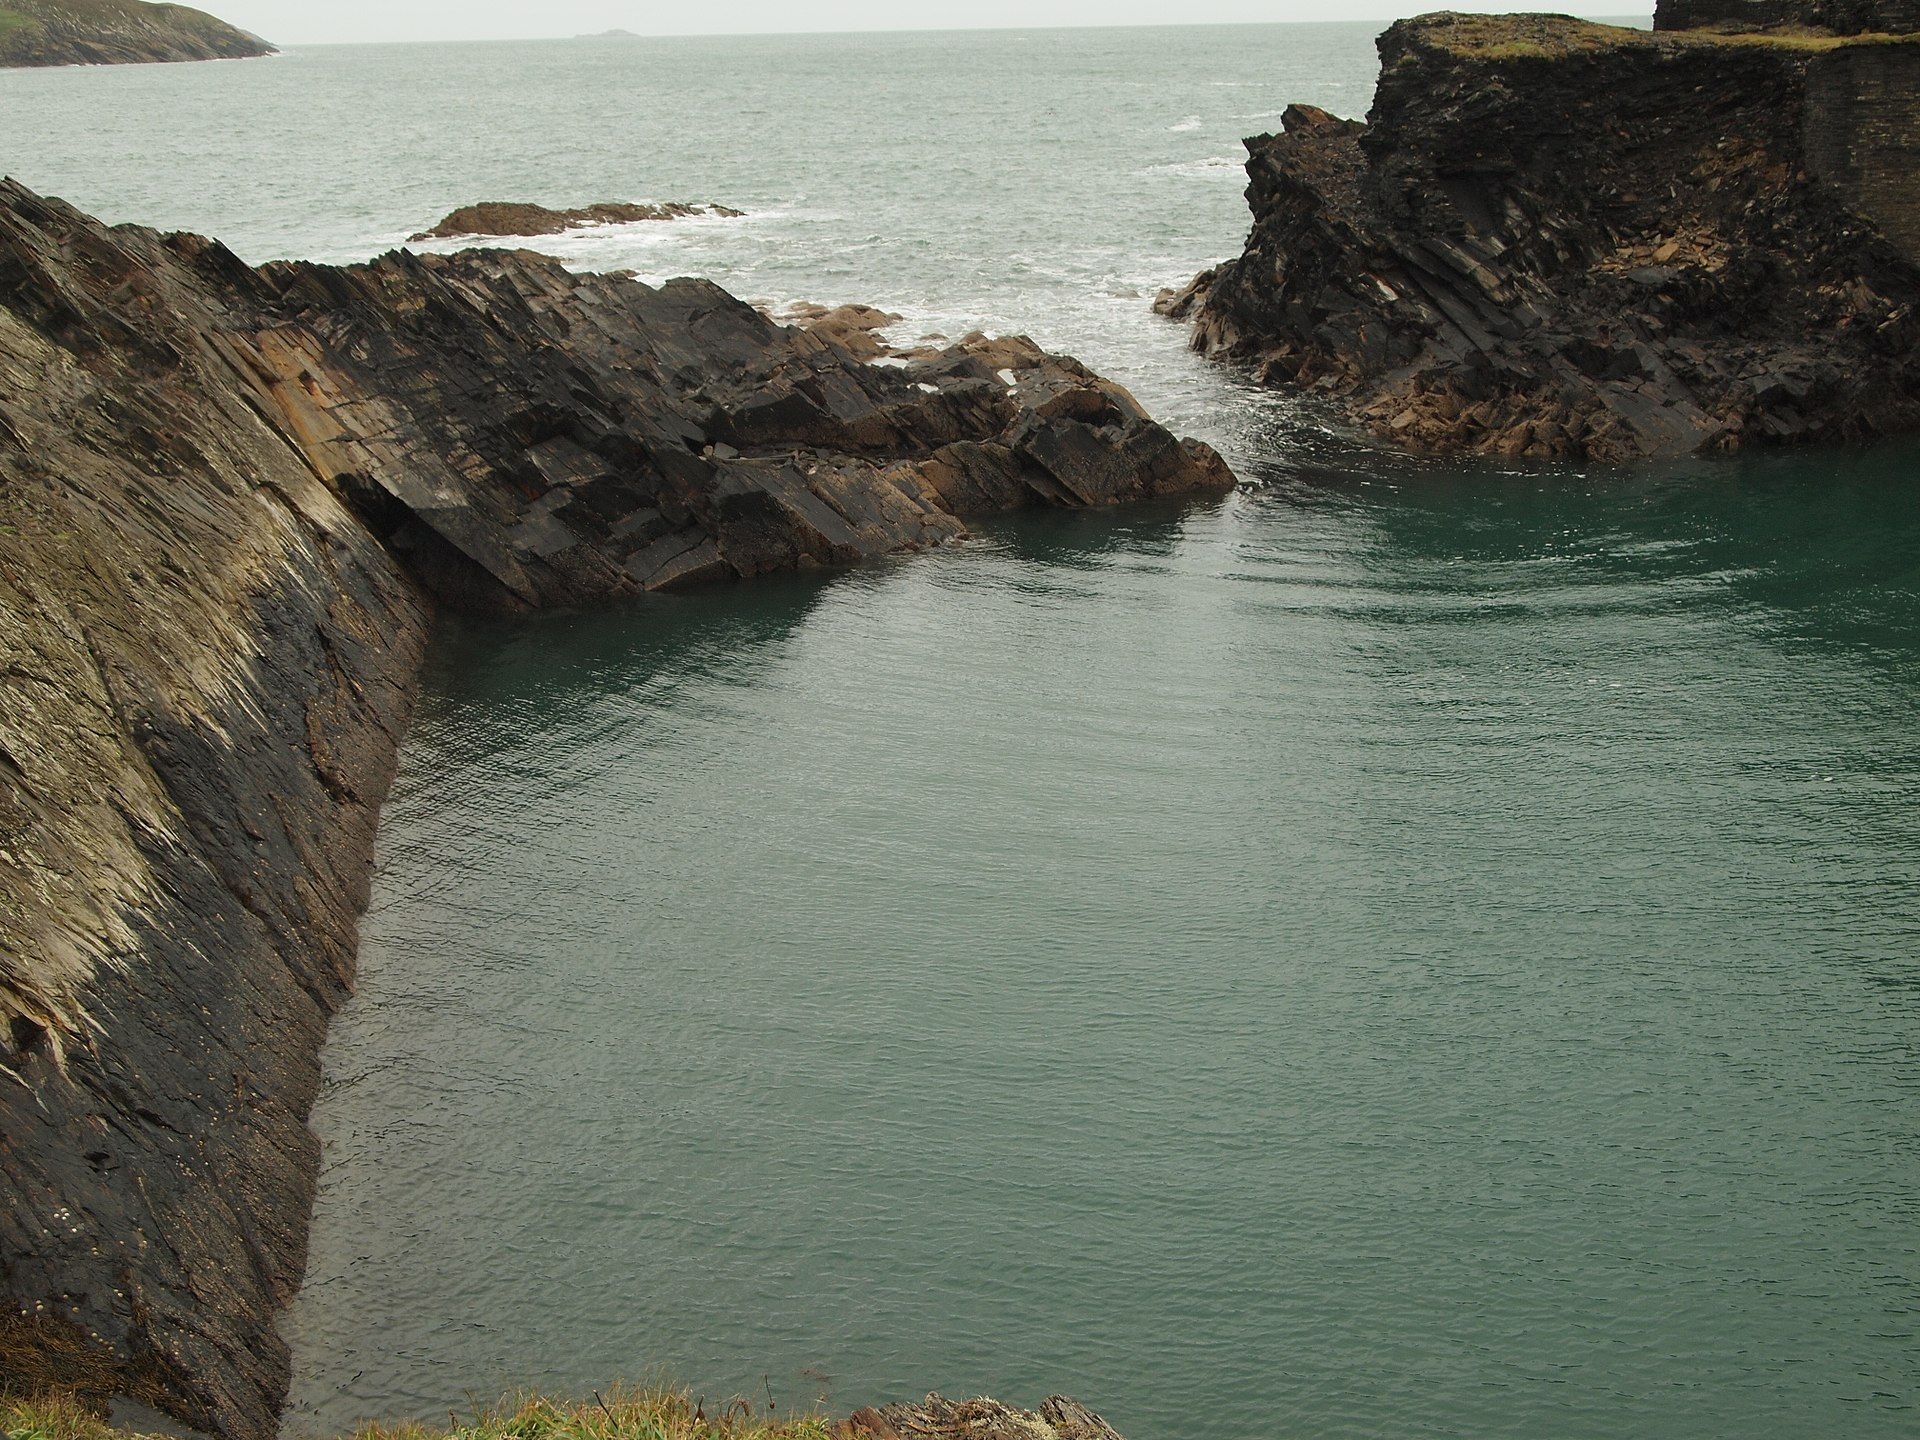
\includegraphics[scale=.11]{diffraction_irl.jpg}
       \caption{Diffraction of water waves through a narrow opening in the shoreline}
       \label{fig:shoreline}
    \end{figure}
\end{frame}

\begin{frame}{Diffraction: Huygens-Fresnel Principle}
    \begin{columns}[T]
        \begin{column}{.45\textwidth}
            This behavior is described by the \alert{Huygens-Fresnel Principle}, which treats each point in the wave as a single spherical wave, whose interference causes the linear wave we see. 
            \begin{figure}
                \centering
                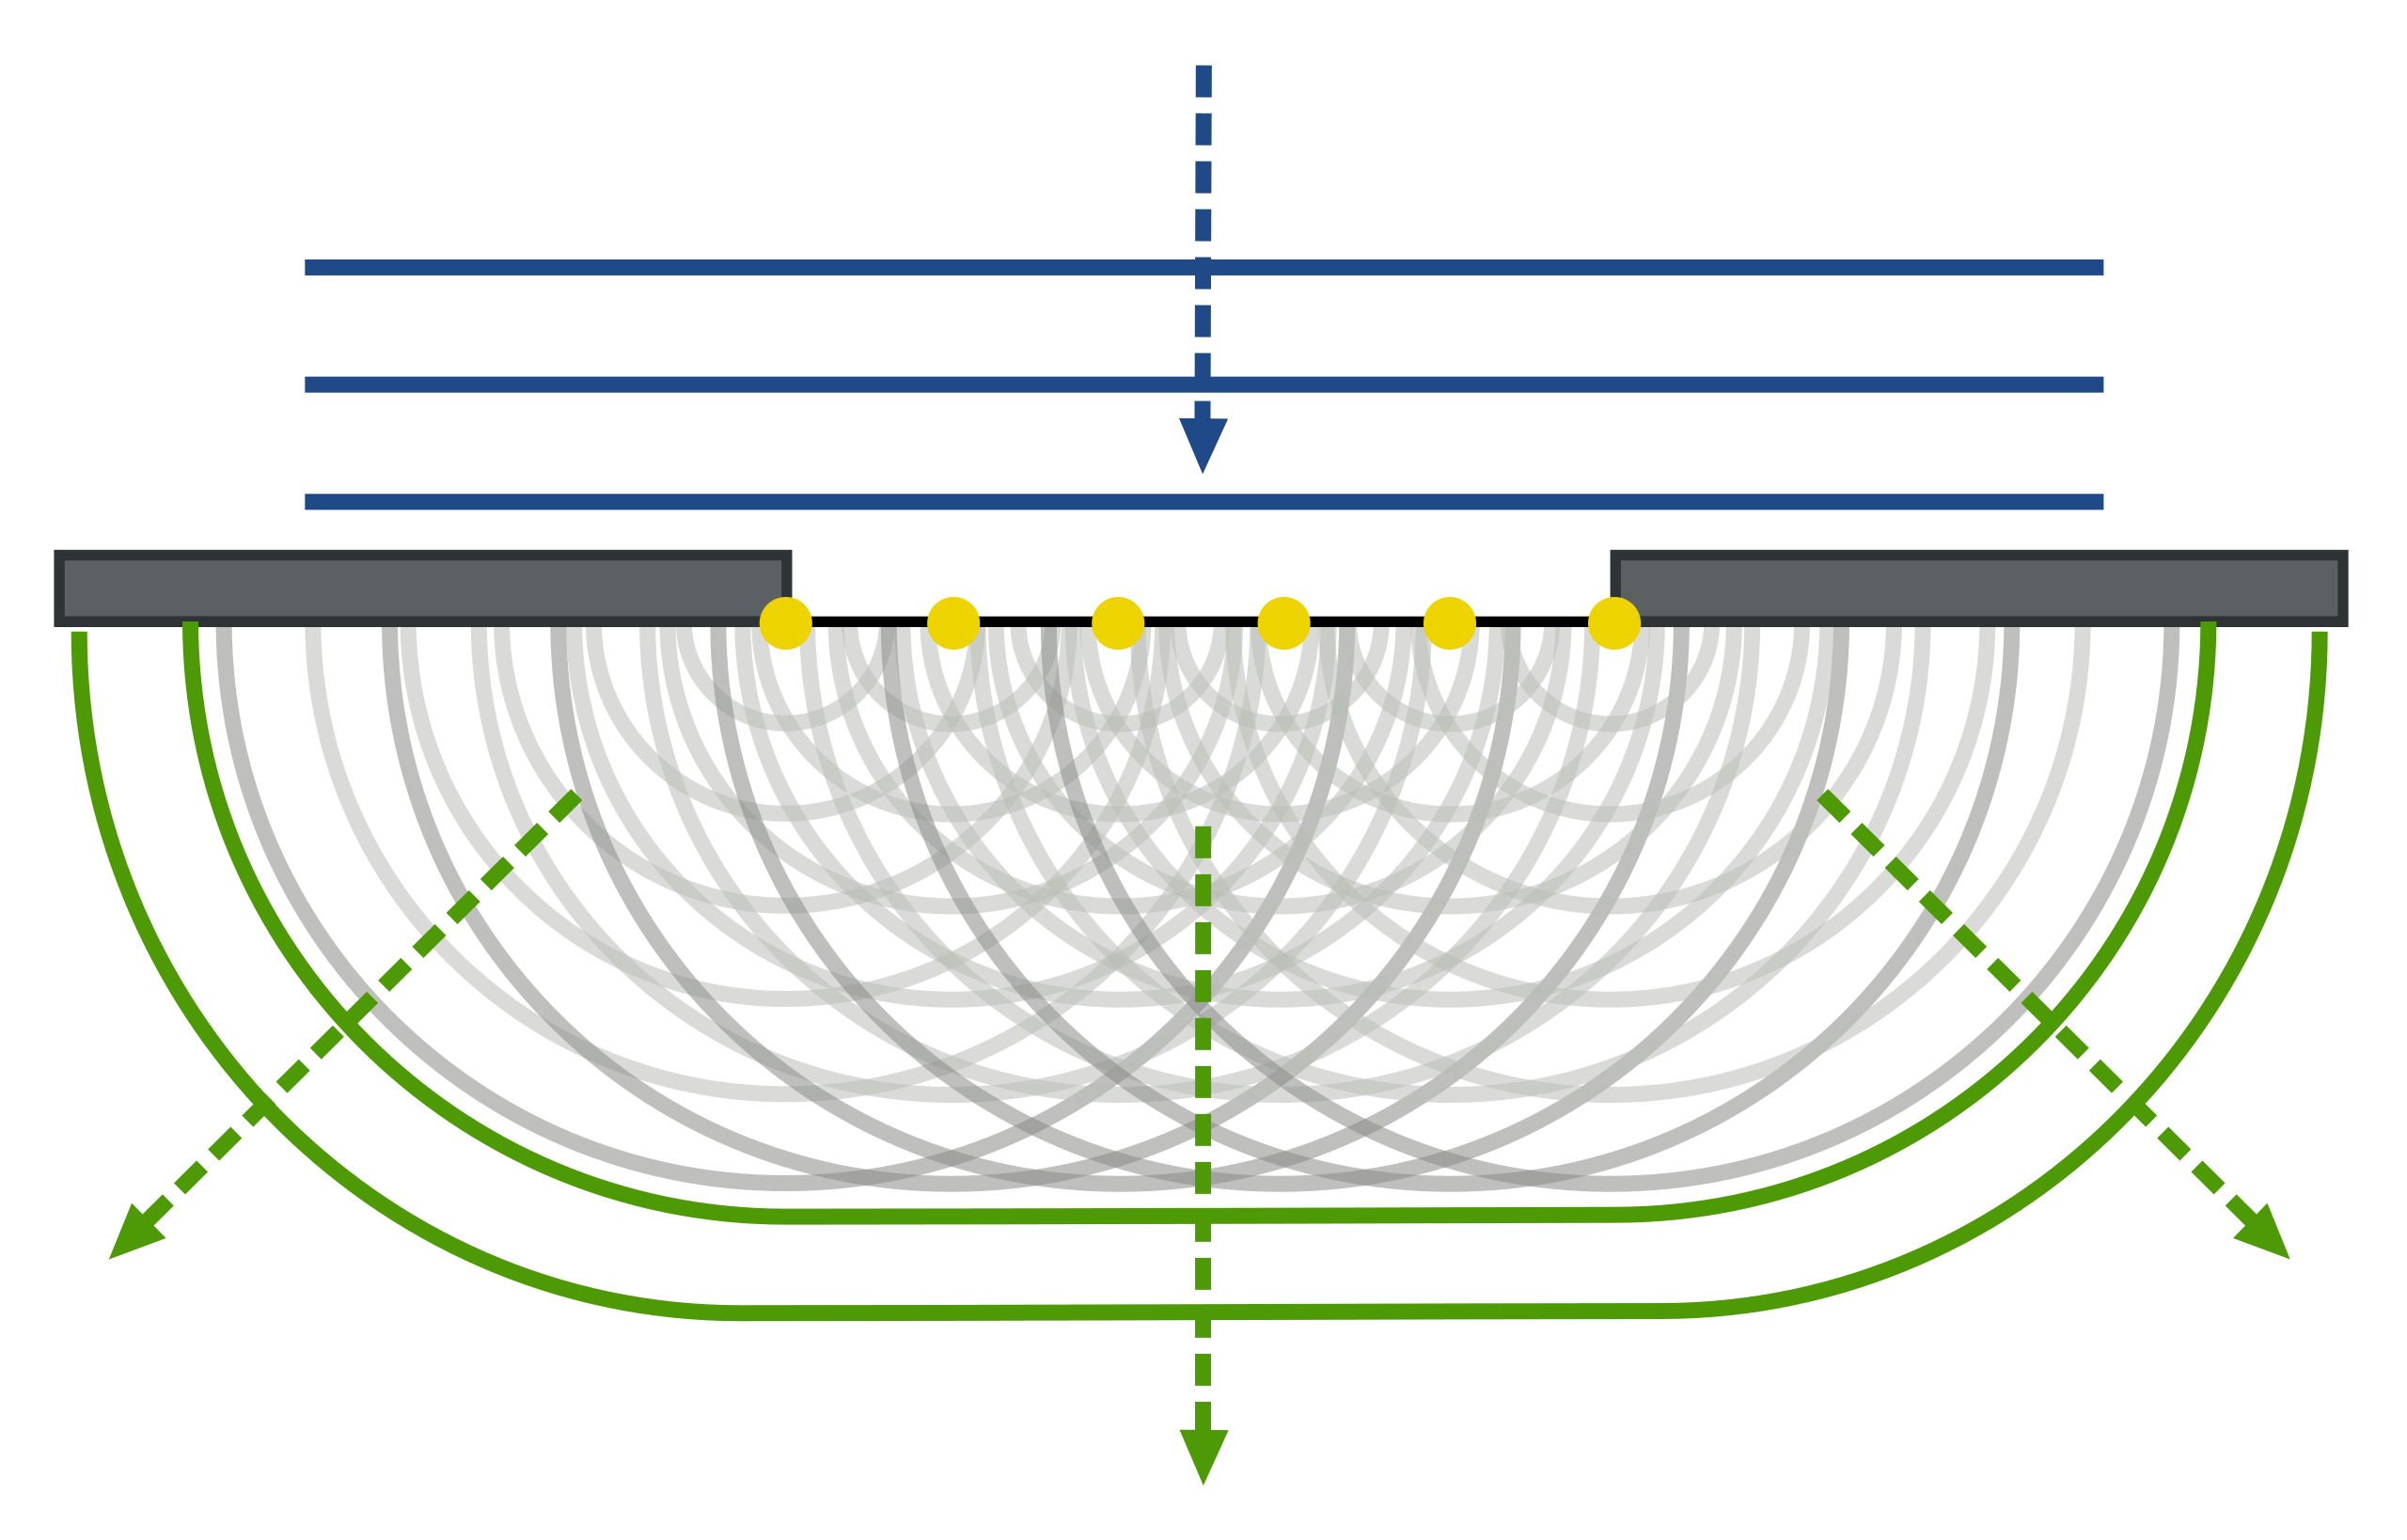
\includegraphics[scale=.05]{huygens.png}
                \caption{Diffraction through a narrow opening as described by Huygen-Fresnel.}
                \label{fig:huygens_diff}
            \end{figure}
        \end{column}
         \begin{column}{.45\textwidth}
           \begin{figure}
               \centering
               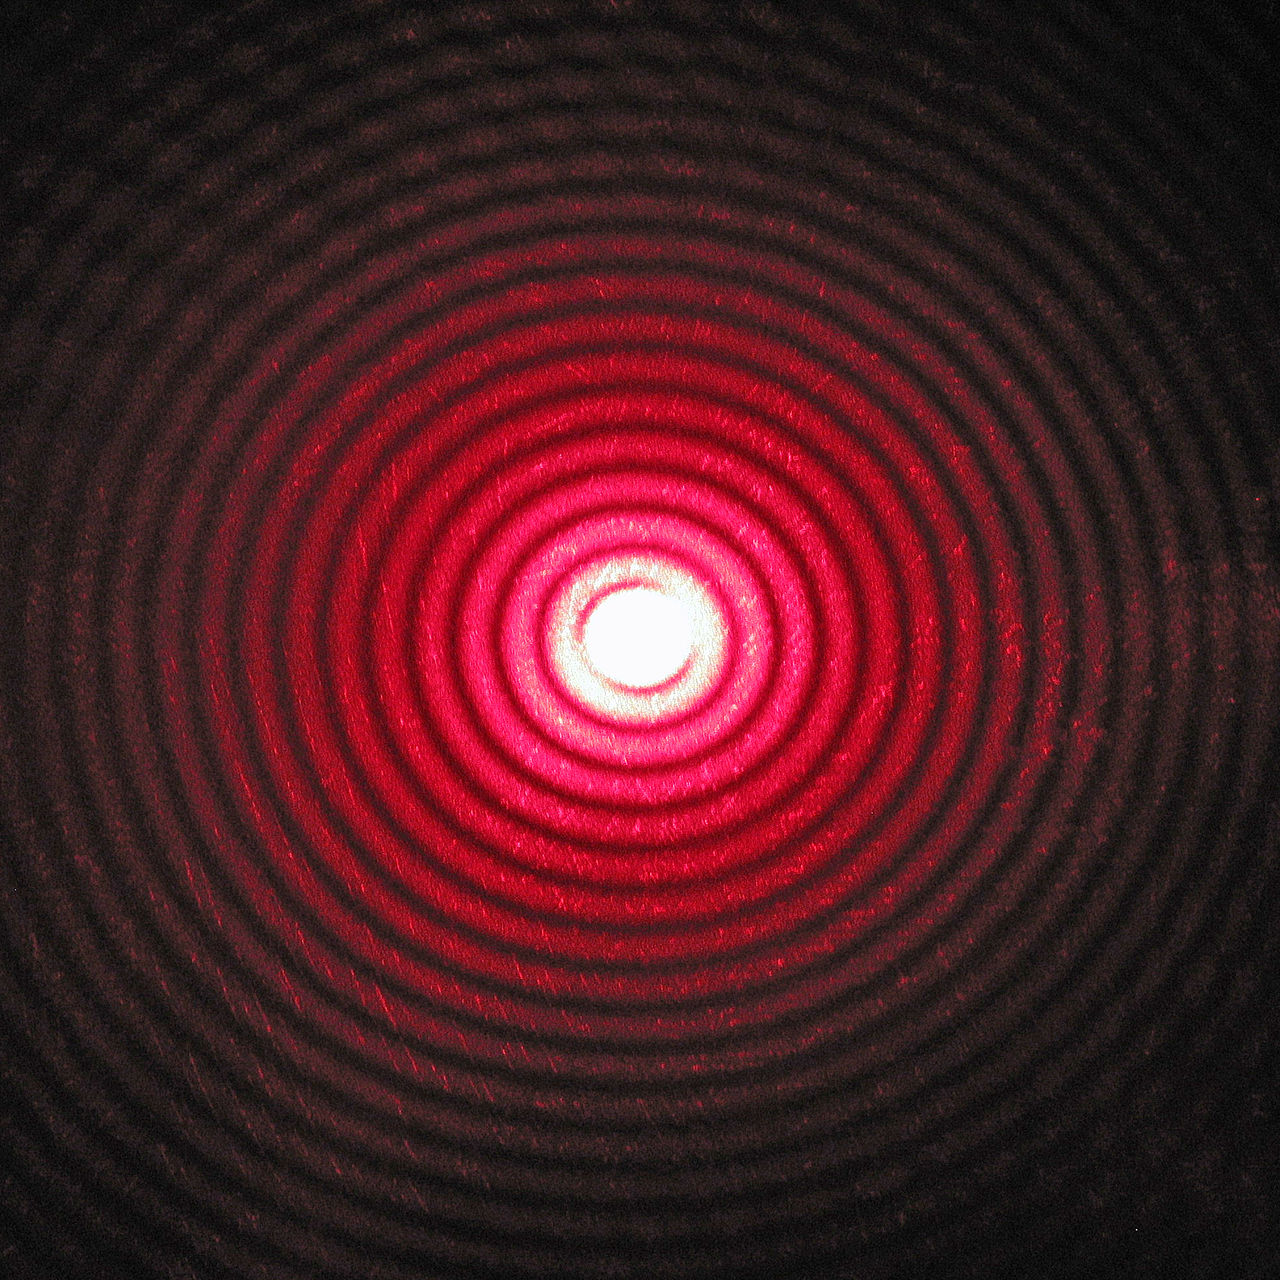
\includegraphics[scale=.26]{laserdiffraction.jpg}
               \caption{Diffraction pattern of a laser beam after passing through a small hole.}
               \label{fig:laserdiff}
           \end{figure}
         \end{column}
    \end{columns}
\end{frame}

\begin{frame}{Linear Source: Diffraction}
    We can create diffraction by adding a small object or slits into the water. \vspace{2mm}
    \begin{columns}[T]
        \begin{column}{.45\textwidth}
            We'll first add a small rectangle to the water pool.
            \begin{itemize}
                \item What do we expect to see in its shadow?
            \end{itemize}
            \begin{figure}
                \centering
                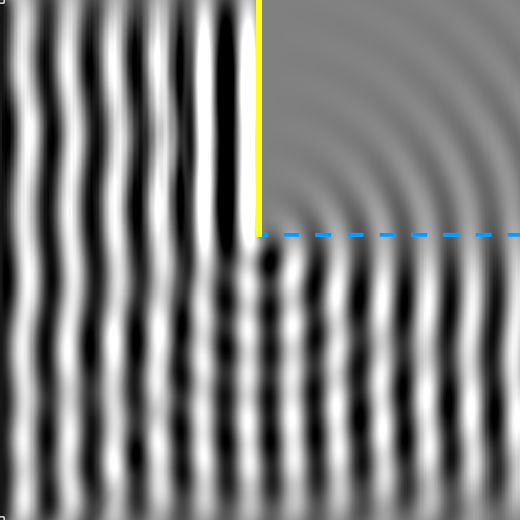
\includegraphics[scale=.2]{ripplediffobj.png}
                \caption{The effect of diffraction on plane waves after being blocked by an object.}
                \label{fig:planediffobject}
            \end{figure}
        \end{column}
         \visible<3->{\begin{column}{.45\textwidth}
           Now, let's use a slit.
           \begin{itemize}
               \item What pattern does diffraction predict?
           \end{itemize}
           \visible<4->{
           \begin{figure}
               \centering
               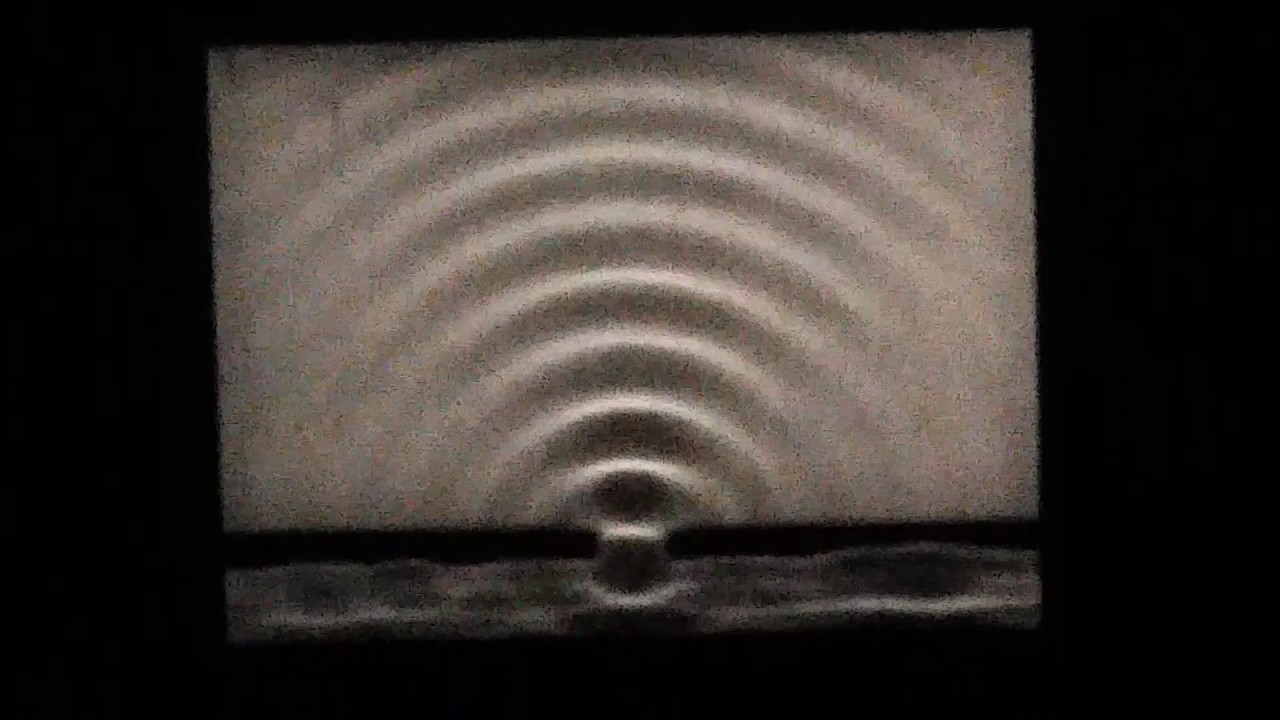
\includegraphics[scale=.1]{ripplediffslit.jpg}
               \caption{Diffraction through a narrow slit.}
               \label{fig:planediffslit}
           \end{figure}
            \vspace{-5mm}
           \begin{itemize}
               \item What if we use several slits?
           \end{itemize}}
         \end{column}}
    \end{columns}
\end{frame}

\begin{frame}{Review: Refraction}
    \alert{Refraction} occurs when a wave passes from one medium to another, causing it to change speed.
    \begin{columns}[T]
        \begin{column}{.45\textwidth}
            \begin{figure}
                \centering
                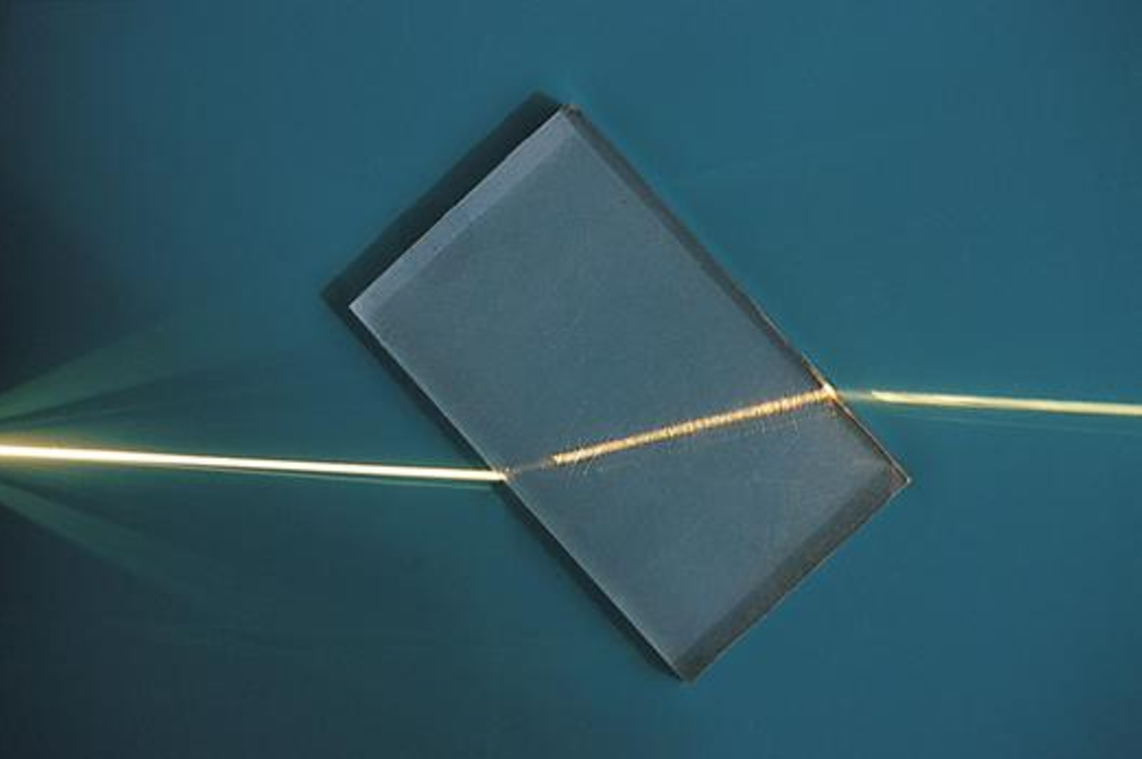
\includegraphics[scale=.25]{refraction1.png}
                \caption{Light refracting through a piece of plastic. The speed of light is different in plastic than in air, so the beam bends.}
                \label{fig:lightdiff}
            \end{figure}
        \end{column}
         \begin{column}{.45\textwidth}
           \begin{figure}
               \centering
               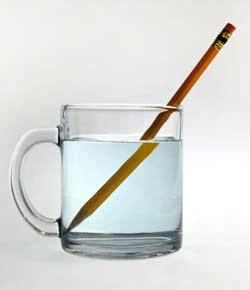
\includegraphics[scale=.4]{pencilref.jpg}
               \caption{The difference in the speed of light in water and air causes the pencil to appear split due to refraction.}
               \label{fig:pendiff}
           \end{figure}
         \end{column}
    \end{columns}
\end{frame}

\begin{frame}{Review: Refraction}
    Refraction causes waves to bend \textit{towards the normal} when they encounter a medium in which they travel slower, and away from the normal when encountering a medium in which they travel faster. 
    
    \begin{figure}
        \centering
        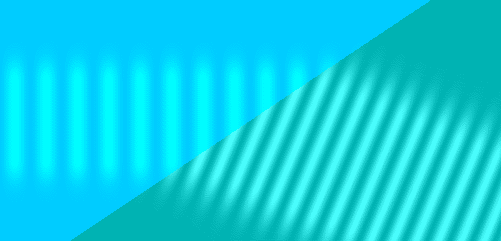
\includegraphics[scale=.6]{refractionwaves.png}
        \caption{Waves travel slower in the new medium and thus must bend to stay connected.}
        \label{fig:refraction_waves}
    \end{figure}
\end{frame}

\begin{frame}{Example: The Beach}
    Water travels slower in shallow water, so waves refract to be perpendicular to the beach as they approach the shore.
    \begin{figure}
        \centering
        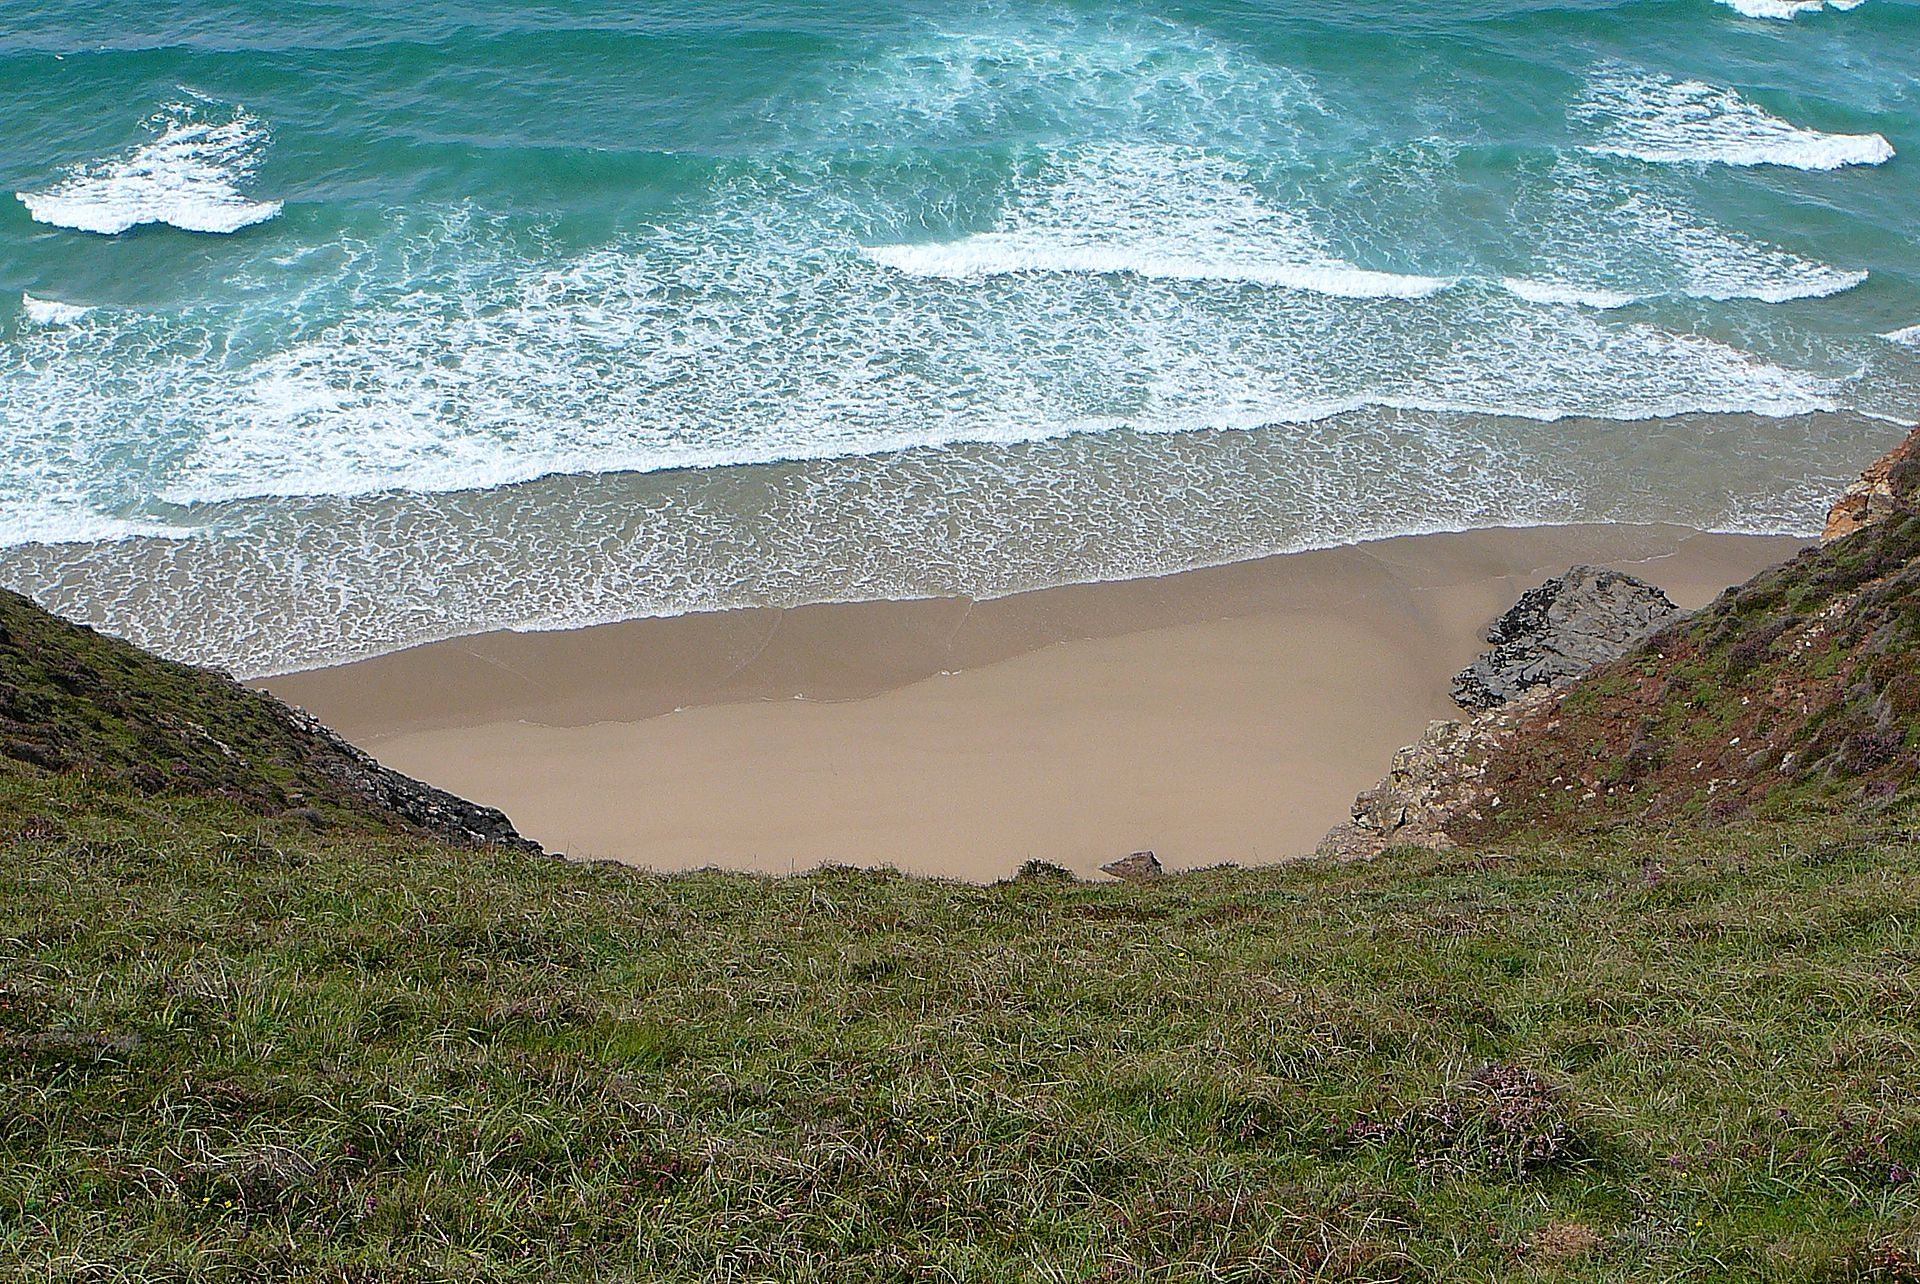
\includegraphics[scale=.11]{waves.jpg}
        \caption{Refraction affecting waves on the beach}
        \label{fig:refraction_beach}
    \end{figure}
\end{frame}

\begin{frame}{Linear Source: Refraction}
    We can add a piece of glass to the bottom of the water pool, making the pool shallower.
    \begin{columns}[T]
        \begin{column}{.45\textwidth}
            \begin{itemize}
                \item What do we expect to see as the water passes over the shallower area?
            \end{itemize}
        \end{column}
         \begin{column}{.45\textwidth}
           \begin{itemize}
                \item When they move from the shallow area back into the deeper area?
            \end{itemize}
         \end{column}
    \end{columns}
    \visible<2->{
    \begin{figure}
        \centering
        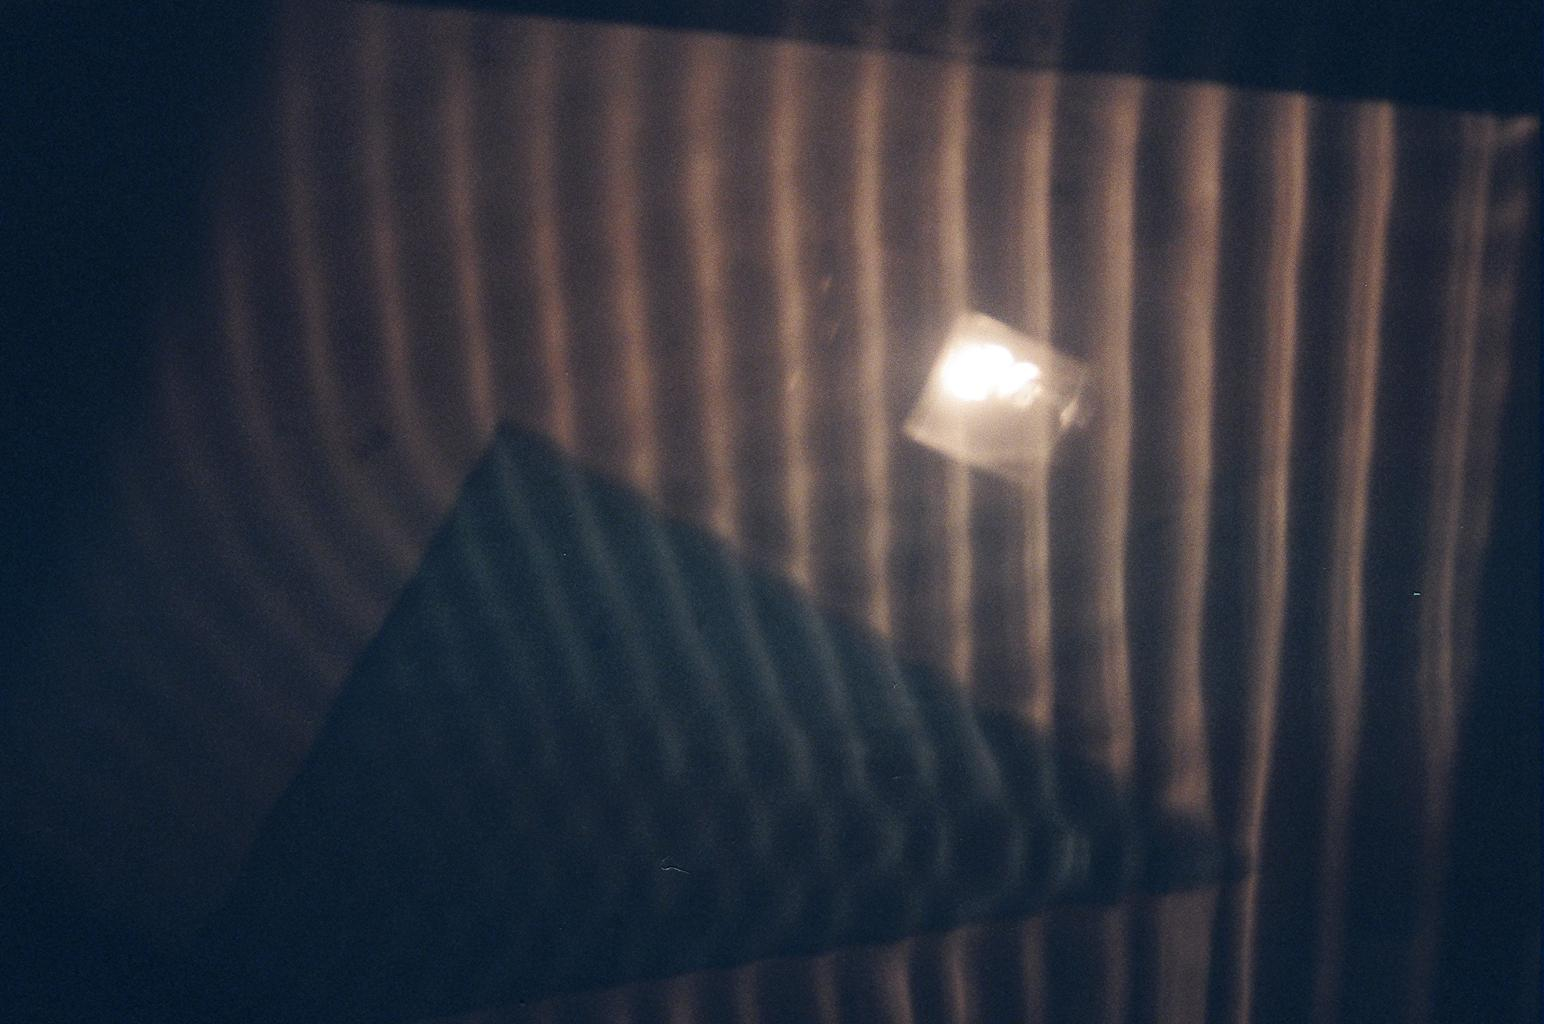
\includegraphics[scale=.12]{ripplerefract.JPG}
        \caption{Refraction over a glass piece in a ripple tank}
        \label{fig:ripple_refract}
    \end{figure}}
\end{frame}

\begin{frame}{Point Source}
    Rather than a plane wave, we can create a radial wave by using a single point as our wave source rather than a bar. What will this look like?
    \visible<2->{\begin{figure}
        \centering
        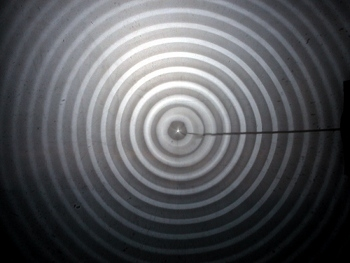
\includegraphics[scale=.5]{radialwaves.jpg}
        \caption{Waves propogating radially from a point source in a ripple tank.}
        \label{fig:radialripples}
    \end{figure}}
\end{frame}

\begin{frame}{Point Source: Reflection off Flat Surface}
We can once again add a flat surface to the tank to see the effect of reflection. What should happen in this case?
\visible<2->{
\begin{figure}
    \centering
    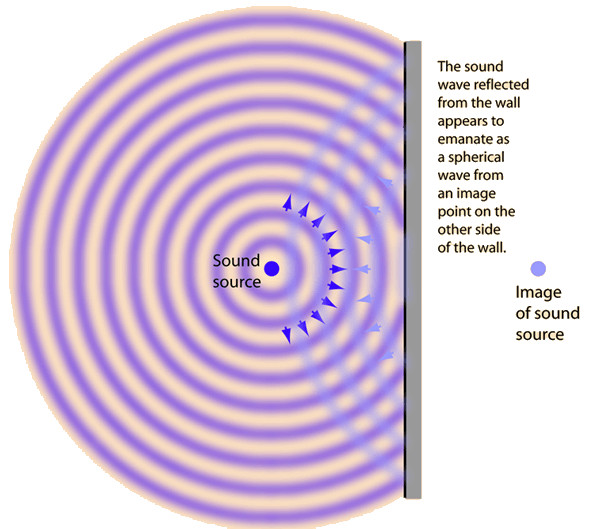
\includegraphics[scale=.3]{wavereflect.png}
    \caption{Radial waves reflecting off a flat surface}
    \label{fig:radialreflect}
\end{figure}}
    
\end{frame}

\begin{frame}{Point Source: Reflection off Parabola}
    Placing a parabola into the water, what should the reflected waves look like? \vspace{5mm}
    
    \visible<2->{This is hard to see in the ripple tank, unfortunately, but if we place the wave source at the \alert{focal point}, they should reflect to form plane waves.}
\end{frame}

\begin{frame}{Two Point Sources: Interference}
    We can add a second point source to see the interference that results. What pattern will be created when the waves overlap?
\end{frame}

\begin{frame}{Point Source: Diffraction}
    Let's follow the same steps as above to see what happens with diffraction.
\end{frame}

\begin{frame}{Try it}
    Does anyone have anything they want to try in the ripple tank?
\end{frame}

\end{document}
